% Provenance (never printed): see sources/outline_sources.md (Year 2: sedimentary basins;
% subsidence curves and backstripping; the stretching model). Stretching model after McKenzie
% (1978) as restated by Sheplev and Reverdatto (1998) and coded in pyBacktrack (EarthByte);
% backstripping after pyBacktrack's well module; North Sea after Sclater and Christie (1980);
% Michigan after Sloss (1982) and Crowe et al. (2009); the US Atlantic margin after Schlee et
% al. (1976), Poag (1979) and Lang et al. (2024); the Molasse after the chapter 13 rows.
% Curves and the invented well from figdata/bachelor-2/basins.py; exercise and problem values
% in the Book 4 scratch calculator calc/ch16.py.
\chapter{Perbandingan Cekungan Sedimen}\label{ch:b2:basins-compared}

Di lepas pantai timur Amerika Serikat, di bawah paparan benua, Baltimore
Canyon Trough menyimpan sedikitnya \qty{14}{km} batuan sedimen. Sumur bor yang menembus tumpukan
seperti itu membaca sejarahnya dari belakang: setiap satuan yang dilaluinya dulu adalah dasar laut, pada kedalaman yang
direkam oleh fosil dan sedimen, dan sejak itu terkubur dan terperas. Kedalaman setiap
permukaan yang berumur diketahui adalah satu titik pada \omterm{def:b2:basins-compared:curve}{kurva penurunan}. Namun sebagian besar penurunan itu disebabkan oleh
berat sedimen itu sendiri. Untuk mengetahui apa yang membentuk cekungan itu, berat tersebut harus diangkat,
lapis demi lapis. Bab ini menunjukkan caranya, dan apa yang dikatakan hasilnya tentang litosfer.
% ledger: poag79:bct, schlee76:atlantic

\begin{recall}
\textbf{Dari volume Tahun 1}: cekungan sedimen, penurunan dan penurunan tektonik,
akomodasi, eustasi; pemadatan, dekompaksi dan hukum Athy, ketebalan padat suatu
lapisan; beban sedimen, yang memperbesar penurunan dengan faktor $(\rho_m - \rho_w)/(\rho_m - \rho_s)$;
isostasi Airy; litosfer dan geotermnya; celah benua dan tepi pasif.
\textbf{Dari buku-buku fisika}: persamaan kalor dan penyelesaian Fourier-nya.
\textbf{Dari \cref{ch:b2:alpine-orogen}}: \omterm{def:b2:alpine-orogen:foreland}{cekungan depan-pegunungan}, \omterm{def:b2:alpine-orogen:foreland}{flysch} dan \omterm{def:b2:alpine-orogen:foreland}{molasse}.
\end{recall}

\begin{omfigure}
\centering
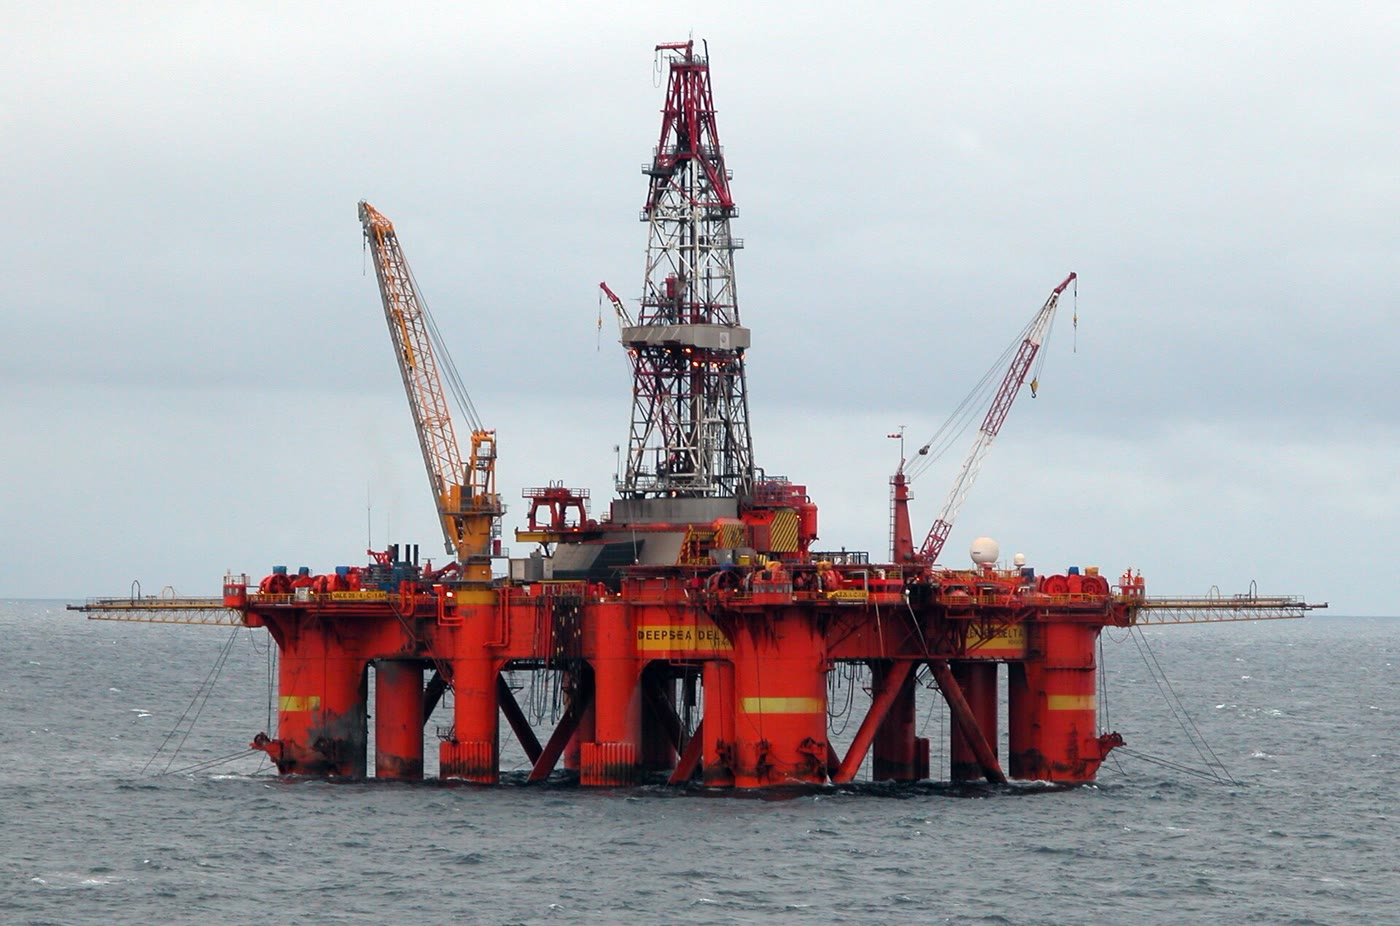
\includegraphics[width=0.66\linewidth]{images/book4/b2-16-drilling-rig.jpg}
\par\smallskip{\small Anjungan pengeboran semi-selam di Laut Utara. Sumur bor yang dibor
dari anjungan seperti itu memberikan ketebalan, umur, dan jenis batuan yang menjadi dasar rekonstruksi penurunan
suatu cekungan. Foto: Erik Christensen, 2005, CC BY-SA 3.0.}
\end{omfigure}

\section{Cekungan dan apa yang membuatnya turun}\label{sec:b2:basins-compared:types}

Volume Tahun 1 membedakan cekungan menurut letaknya. Di sini cekungan dibedakan menurut apa yang menggerakkan
penurunannya.

\begin{definition}[Cekungan intrakratonik, cekungan celah, dan cekungan tepi pasif]\label{def:b2:basins-compared:types}
Yang disebut \emph{cekungan intrakratonik}\index{cekungan intrakratonik} adalah cekungan yang luas, bundar atau lonjong di
bagian dalam benua, jauh dari batas lempeng, yang turun perlahan selama waktu yang sangat panjang
tanpa pensesaran besar. Yang disebut \emph{cekungan celah}\index{cekungan celah} adalah cekungan yang dibatasi sesar normal
dalam litosfer benua yang sedang diregangkan; penurunannya mengikuti peregangan dan kemudian
pendinginan litosfer itu. Yang disebut \emph{cekungan tepi pasif}\index{cekungan tepi pasif} adalah
baji sedimen, yang menebal ke arah samudra, yang terakumulasi di tepi benua setelah
pemisahan benua, di atas kerak yang menipis dari celah lama.
\end{definition}

\omterm{def:b2:alpine-orogen:foreland}{Cekungan depan-pegunungan} dari \cref{ch:b2:alpine-orogen} melengkapi daftar itu, dan cekungan yang membuka
di sepanjang sesar geser-mendatar diserahkan kepada volume Tahun 3. Tiga mekanisme membuat dasar
cekungan turun:
\begin{itemize}
  \item penipisan \emph{mekanis}: ketika kerak diregangkan dan ditipiskan oleh sesar-sesar, kerak yang ringan
        digantikan oleh mantel yang lebih padat dan permukaan turun untuk memulihkan isostasi;
  \item kontraksi \emph{termal}: litosfer yang telah dipanaskan, oleh peregangan atau dari
        bawah, lalu mendingin, menjadi lebih padat dan turun, perlahan, selama puluhan juta tahun;
  \item \emph{pembebanan}: berat sabuk sesar dorong, atau berat sedimen itu sendiri, melengkungkan
        litosfer ke bawah; fleksur itu termasuk volume Tahun 3, dan bentuk lokal beban sedimen, yaitu bentuk
        Airy, sudah cukup di sini.
\end{itemize}
\omterm{def:b2:basins-compared:types}{Cekungan celah} menggabungkan dua mekanisme pertama, tepi pasif mewarisi mekanisme kedua dari tahap celahnya,
\omterm{def:b2:alpine-orogen:foreland}{cekungan depan-pegunungan} dibuat oleh mekanisme ketiga. \omterm{def:b2:basins-compared:types}{Cekungan intrakratonik} adalah yang paling sedikit dipahami.

\begin{omfigure}
\centering
\begin{tikzpicture}[x=1cm, y=1cm, font=\scriptsize, line join=round,
  sed/.style={fill=yellow!35, draw=black!60, line width=0.3pt},
  crust/.style={fill=orange!25, draw=black!60, line width=0.3pt},
  mlith/.style={fill=green!12, draw=black!60, line width=0.3pt},
  asth/.style={fill=red!12, draw=black!60, line width=0.3pt},
  sea/.style={fill=blue!8, draw=none},
  ttl/.style={anchor=south west, font=\scriptsize\bfseries}]
% (a) intracratonic
\begin{scope}
\fill[asth] (0,-2.4) rectangle (6.6,-1.6);
\fill[mlith] (0,-1.6) rectangle (6.6,-0.7);
\fill[crust] (0,-0.7) -- (6.6,-0.7) -- (6.6,0) -- (4.9,0) .. controls (4.1,-0.45) and (2.5,-0.45) .. (1.7,0) -- (0,0) -- cycle;
\fill[sed] (1.7,0) .. controls (2.5,-0.45) and (4.1,-0.45) .. (4.9,0) -- cycle;
\draw[black!70] (0,0) -- (6.6,0);
\node[ttl] at (0,0.05) {(a) intrakratonik};
\node at (3.3,-1.15) {litosfer mantel};
\node at (3.3,-2.0) {astenosfer};
\end{scope}
% (b) rift
\begin{scope}[xshift=7.2cm]
\fill[asth] (0,-2.4) -- (6.6,-2.4) -- (6.6,-1.6) -- (4.5,-1.6) -- (3.3,-1.0) -- (2.1,-1.6) -- (0,-1.6) -- cycle;
\fill[mlith] (0,-1.6) -- (2.1,-1.6) -- (3.3,-1.0) -- (4.5,-1.6) -- (6.6,-1.6) -- (6.6,-0.7) -- (4.4,-0.7) -- (3.3,-0.45) -- (2.2,-0.7) -- (0,-0.7) -- cycle;
\fill[crust] (0,-0.7) -- (2.2,-0.7) -- (3.3,-0.45) -- (4.4,-0.7) -- (6.6,-0.7) -- (6.6,0) -- (4.6,0) -- (4.25,-0.42) -- (3.75,-0.2) -- (3.35,-0.4) -- (2.95,-0.15) -- (2.45,-0.42) -- (2.0,0) -- (0,0) -- cycle;
\fill[sed] (2.0,0) -- (2.45,-0.42) -- (2.95,-0.15) -- (3.35,-0.4) -- (3.75,-0.2) -- (4.25,-0.42) -- (4.6,0) -- cycle;
\draw[thick] (2.0,0) -- (2.5,-0.5) (4.6,0) -- (4.2,-0.5) (2.95,-0.15) -- (3.4,-0.48);
\draw[black!70] (0,0) -- (6.6,0);
\node[ttl] at (0,0.05) {(b) celah};
\node at (1.45,-1.15) {litosfer mantel};
\node at (5.4,-2.0) {astenosfer};
\end{scope}
% (c) passive margin
\begin{scope}[yshift=-3.3cm]
\fill[asth] (0,-2.4) -- (6.6,-2.4) -- (6.6,-1.2) -- (0,-1.6) -- cycle;
\fill[mlith] (0,-1.6) -- (6.6,-1.2) -- (6.6,-1.0) -- (4.2,-1.05) -- (2.4,-0.75) -- (0,-0.7) -- cycle;
\fill[crust] (0,-0.7) -- (2.4,-0.75) -- (4.2,-1.05) -- (4.2,-0.85) -- (2.6,-0.25) -- (1.6,0) -- (0,0) -- cycle;
\fill[gray!35, draw=black!60, line width=0.3pt] (4.2,-1.05) -- (6.6,-1.0) -- (6.6,-0.85) -- (4.2,-0.85) -- cycle;
\fill[sed] (1.6,0) -- (2.6,-0.25) -- (4.2,-0.85) -- (6.6,-0.85) -- (6.6,-0.55) -- (3.6,-0.45) -- (2.6,-0.05) -- (2.2,0) -- cycle;
\fill[sea] (2.2,0) -- (6.6,0) -- (6.6,-0.55) -- (3.6,-0.45) -- (2.6,-0.05) -- cycle;
\draw[black!70] (0,0) -- (2.2,0);
\draw[blue!60!black] (2.2,0) -- (6.6,0);
\node[ttl] at (0,0.05) {(c) tepi pasif};
\node at (5.4,-0.95) {\tiny kerak samudra};
\node at (1.3,-2.0) {astenosfer};
\node at (1.3,-1.05) {litosfer mantel};
\end{scope}
% (d) foreland
\begin{scope}[xshift=7.2cm, yshift=-3.3cm]
\fill[asth] (0,-2.4) -- (6.6,-2.4) -- (6.6,-2.0) -- (0,-1.5) -- cycle;
\fill[mlith] (0,-1.5) -- (6.6,-2.0) -- (6.6,-1.2) -- (0,-0.7) -- cycle;
\fill[crust] (0,-0.7) -- (6.6,-1.2) -- (6.6,-0.55) -- (3.6,-0.4) .. controls (2.0,-0.15) .. (0,0) -- cycle;
\fill[sed] (0,0) .. controls (2.0,-0.15) .. (3.6,-0.4) -- (6.6,-0.55) -- (5.0,0) -- cycle;
\fill[crust, fill=orange!45] (5.0,0) -- (6.6,-0.55) -- (6.6,0.6) -- (6.1,0.6) -- cycle;
\draw[thrust fault] (6.6,-0.55) -- (5.0,0);
\draw[black!70] (0,0) -- (5.0,0);
\node[ttl] at (0,0.05) {(d) depan-pegunungan};
\node[anchor=north east, font=\tiny] at (6.55,0.55) {sabuk};
\node at (2.2,-1.25) {litosfer mantel};
\node at (1.5,-2.05) {astenosfer};
\end{scope}
\end{tikzpicture}
\par\smallskip{\small Empat keluarga cekungan dalam penampang skematis melintasi litosfer (tidak
berskala; sedimen berwarna kuning, kerak benua berwarna jingga, dan kerak samudra berwarna kelabu). Pembesaran vertikalnya
besar: cekungan yang sebenarnya selebar ratusan kilometer dan sedalam beberapa sampai lima belas
kilometer.}
\end{omfigure}

Cekungan-cekungan celah Laut Utara adalah kasus klasik dua mekanisme pertama. Graben-graben
terbentuk di sana sejak Trias, dan peregangan besar terakhir berlangsung dari Jura Tengah
sampai pertengahan Kapur; sesar-sesar lalu tenang, dan bagian tengah cekungan terus turun
sebagai piring yang lebar, yang terisi oleh kapur, batu pasir dan, selama sebagian besar Tersier, serpih dan
batu lumpur. Jika dibebani air saja, batuan dasarnya akan turun lagi 1100 sampai
\qty{1400}{m} di bagian tengah dan 600 sampai \qty{700}{m} di sayap-sayapnya setelah pensesaran berhenti.
% ledger: sc80b4:north-sea

Tepi pasif Amerika Serikat bagian timur menunjukkan penurunan yang sama dalam skala yang lebih besar.
Profil seismik yang melintasi paparan menunjukkan lebih dari \qty{14}{km} batuan Mesozoikum dan yang lebih muda di
Baltimore Canyon Trough dan \qty{8}{km} di cekungan Georges Bank, dalam satuan-satuan yang menebal
ke arah samudra. Pusat-pusat pengendapan Jura-nya mengikuti struktur celah dan zona-zona
penurunan termalnya yang kemudian.
% ledger: schlee76:atlantic, lang24:atlantic

Cekungan Michigan adalah tipe \omterm{def:b2:basins-compared:types}{cekungan intrakratonik}. Berbentuk lonjong, dengan luas beberapa ratus ribu
kilometer persegi, cekungan itu menyimpan lebih dari \qty{4}{km} sedimen Fanerozoikum yang diendapkan
dalam episode-episode terpisah selama sekitar 500 juta tahun, dengan sedikit pensesaran. Episode-episode
penurunannya yang lebih cepat bertepatan dengan episode cekungan lain di bagian dalam Amerika Utara dan benua-benua
lain, yang mengisyaratkan penyebab yang lebih besar daripada satu cekungan. \omterm{def:b2:basins-compared:backstripping}{Pengupasan balik} lebih dari 57\,000
log sumur menunjukkan pola penurunan yang berumur panjang dan hampir melingkar, yang menurut para penulisnya dapat dijelaskan oleh
aliran turun mantel, yang terputus pada waktu dua orogenesis di tepi
benua yang jauh. Mengapa \omterm{def:b2:basins-compared:types}{cekungan intrakratonik} turun masih diperdebatkan.
% ledger: sloss82:michigan, crowe09:michigan

\section{Kurva penurunan}\label{sec:b2:basins-compared:curves}

Sebuah sumur, atau penampang terukur, memberikan untuk setiap satuan kedalamannya kini, jenis batuannya, dan umurnya,
yang dibaca dari fosil atau dari korelasi. Bersama kedalaman air tempat setiap satuan
diendapkan, yang dibaca dari fosil dan struktur sedimennya, data itu memberikan sejarah cekungan.

\begin{definition}[Kurva penurunan]\label{def:b2:basins-compared:curve}
Yang disebut \emph{kurva penurunan}\index{kurva penurunan} suatu cekungan di suatu tempat adalah grafik kedalaman
permukaan acuan, biasanya batuan dasar atau dasar satuan tertua, di bawah muka laut,
terhadap waktu. Kurva penurunan \emph{total} memakai tebal sedimen sebagaimana adanya pada setiap
waktu, ditambah kedalaman air; kurva penurunan \emph{tektonik} menggantikan sedimen dengan air
dan menghilangkan efek isostatiknya.
\end{definition}

Suatu satuan tidak pernah setebal di masa lalu seperti kini. Saat terkubur, satuan itu kehilangan porositas; butirannya tidak
berubah, tetapi airnya telah terperas keluar. Volume Tahun 1 menulis porositas pada kedalaman
$z$ sebagai hukum Athy, $\phi(z) = \phi_0\,e^{-z/c}$, dan menemukan ketebalan padat suatu lapisan di antara
$z_1$ dan $z_2$,
\[
  T_s = (z_2 - z_1) - \phi_0 c\left(e^{-z_1/c} - e^{-z_2/c}\right),
\]
yang tetap sama ketika lapisan itu berpindah. Untuk \emph{mendekompaksi} suatu satuan ke posisi yang lebih dangkal,
dengan puncaknya kini pada $z_1'$, dicarilah dasar $z_2'$ yang menyimpan ketebalan padat yang sama.
Persamaan itu tidak memiliki penyelesaian tertutup, tetapi iterasi titik tetap
\[
  z_2' \leftarrow z_1' + T_s + \phi_0 c\left(e^{-z_1'/c} - e^{-z_2'/c}\right)
\]
dimulai dari $z_2' = z_1' + T_s$ konvergen dalam beberapa langkah. Massa per satuan luas lapisan itu
adalah massa butirannya ditambah massa air porinya,
\[
  m = \rho_g T_s + \rho_w\,(z_2 - z_1 - T_s),
\]
dengan $\rho_g$ massa jenis butiran; membagi massa suatu kolom dengan tebalnya memberikan
massa jenis rata-ratanya $\bar\rho_s$.

Untuk litologi yang dipakai dalam bab ini, pasir, serpih, kapur, dan pasir lempungan, tabel di bawah
memberikan tetapan dari Sclater dan Christie (1980), sebagaimana disertakan dalam sebuah program sumber terbuka.
Pasir mempertahankan porositasnya paling dalam, kapur kehilangan porositasnya paling cepat.
% ledger: pybacktrack:compaction

\begin{center}
\small
\begin{tabular}{lccc}
\hline
litologi & massa jenis butiran (\unit{kg.m^{-3}}) & porositas permukaan $\phi_0$ & panjang peluruhan $c$ (\unit{m}) \\
\hline
pasir & 2650 & 0.49 & 3704 \\
serpih & 2700 & 0.63 & 1960 \\
kapur & 2710 & 0.70 & 1408 \\
pasir lempungan & 2680 & 0.56 & 2564 \\
\hline
\end{tabular}
\end{center}

\section{Pengupasan balik}\label{sec:b2:basins-compared:backstripping}

\omterm{def:b2:basins-compared:curve}{Kurva penurunan} total mencampurkan dua penyebab: apa pun yang membentuk cekungan, dan berat apa yang
mengisinya. Memisahkan keduanya adalah tujuan prosedur berikut, alat utama analisis
cekungan.

\begin{definition}[Pengupasan balik]\label{def:b2:basins-compared:backstripping}
Yang disebut \emph{pengupasan balik}\index{pengupasan balik} (\textit{backstripping}) adalah rekonstruksi penurunan tektonik suatu
cekungan sepanjang waktu: satuan-satuan sebuah sumur diangkat satu per satu, mulai dari yang termuda, satuan-satuan
yang tersisa didekompaksi pada setiap langkah, dan efek isostatik beban sedimen dan air
dihilangkan untuk memberikan kedalaman yang akan dicapai batuan dasar di bawah beban air saja.
\end{definition}

Langkah terakhir adalah keseimbangan isostatik. Volume Tahun 1 membuatnya untuk cekungan yang terisi sampai muka laut;
kasus umumnya menambahkan kedalaman air dan ketinggian muka laut.

\begin{proposition}[Pengupasan balik Airy]\label{prop:b2:basins-compared:backstrip}
Misalkan sebuah cekungan menyimpan, pada suatu waktu, kolom sedimen setebal $S$ dengan massa jenis rata-rata
$\bar\rho_s$, di bawah kedalaman air $W_d$, sementara muka laut berada $\Delta_{SL}$ di atas ketinggiannya kini.
Dalam isostasi lokal di atas mantel bermassa jenis $\rho_m$, dengan air bermassa jenis $\rho_w$,
penurunan tektonik pada waktu itu, diukur dari muka laut kini, adalah
\[
  Y = S\,\frac{\rho_m - \bar\rho_s}{\rho_m - \rho_w} + W_d
      - \Delta_{SL}\,\frac{\rho_m}{\rho_m - \rho_w}.
\]
\end{proposition}

\begin{proof}
Bandingkan dua kolom di atas litosfer yang sama, sampai kedalaman kompensasi di bawah keduanya. Pada
kolom pertama, air sedalam $W_d$ terletak di atas sedimen setebal $S$; pada kolom kedua, air
saja mengisi cekungan sedalam $Y'$ di bawah permukaan laut yang sama. Massa keduanya sama:
\[
  \rho_w W_d + \bar\rho_s S + \rho_m\,(d - W_d - S) = \rho_w Y' + \rho_m\,(d - Y'),
\]
dengan $d$ kedalaman bersama aras kompensasi di bawah permukaan laut. Jadi
$Y'(\rho_m - \rho_w) = S(\rho_m - \bar\rho_s) + W_d(\rho_m - \rho_w)$, yang merupakan dua suku
pertama. Jika muka laut berada $\Delta_{SL}$ lebih tinggi daripada kini, air tambahan itu bukan bagian dari
penurunan cekungan itu sendiri: jika air itu dihilangkan, batuan dasar yang terbebani air naik sebesar
$\Delta_{SL}\rho_w/(\rho_m - \rho_w)$, dan kedalamannya di bawah muka laut kini lebih kecil lagi sebesar
$\Delta_{SL}$; bersama-sama, $\Delta_{SL}\,\rho_m/(\rho_m - \rho_w)$.
\end{proof}
% ledger: pybacktrack:backstrip

Dengan $\rho_m = \qty{3330}{kg.m^{-3}}$ dan $\rho_w = \qty{1030}{kg.m^{-3}}$, kolom sedimen dengan
massa jenis rata-rata \qty{2300}{kg.m^{-3}} dihitung sebesar $1030/2300 = 0.45$ tebalnya dalam penurunan
tektonik: lebih dari separuh tebal isian suatu cekungan diberi ruang oleh beratnya sendiri.
Muka laut yang \qty{100}{m} lebih tinggi daripada kini menurunkan hasilnya sebesar \qty{145}{m}. Kedalaman air dan
muka laut masa lalu adalah data yang paling lemah: fosil memberikan rentang kedalaman air, yang sering selebar ratusan
meter di lereng, dan penurunan tektonik mewarisi rentang itu.

\begin{method}[Pengupasan balik sebuah sumur]\label{met:b2:basins-compared:backstrip}
\begin{enumerate}
  \item Daftarlah satuan-satuan mulai dari dasar, dengan kedalaman puncak dan dasarnya kini,
        tetapan litologinya $(\rho_g, \phi_0, c)$, umur puncaknya, dan kedalaman air pada
        setiap umur itu.
  \item Hitunglah ketebalan padat $T_s$ setiap satuan dari kedalamannya kini.
  \item Untuk umur puncak satuan $k$, angkat semua satuan yang lebih muda. Letakkan puncak satuan
        $k$ pada kedalaman nol dan dekompaksi satuan itu; letakkan setiap satuan yang lebih tua, berturut-turut, di bawah satuan di atasnya
        dan dekompaksi.
  \item Jumlahkan tebal-tebalnya untuk memperoleh $S$, dan massa-massanya untuk memperoleh massa jenis rata-rata
        $\bar\rho_s = \sum m / S$.
  \item Terapkan \cref{prop:b2:basins-compared:backstrip} untuk memperoleh $Y$; penurunan totalnya adalah
        $S + W_d$.
  \item Ulangi untuk setiap umur, dari yang tertua sampai kini; plotkan $Y$ dan $S + W_d$ terhadap umur.
\end{enumerate}
\end{method}

Gambar di bawah menunjukkan hasilnya untuk sebuah sumur rekaan di \omterm{def:b2:basins-compared:types}{cekungan celah}. Empat satuan diambil intinya:
pasir sin-celah yang diendapkan selagi sesar-sesar aktif, antara 165 dan \qty{150}{Ma}; lalu serpih,
kapur, dan pasir lempungan. Kini tidak diperlukan dekompaksi: batuan dasar terletak pada \qty{6030}{m}
dan kolom itu bermassa jenis rata-rata \qty{2358}{kg.m^{-3}}, sehingga $Y = \qty{2648}{m}$ di bawah
\qty{100}{m} air. Pada \qty{150}{Ma}, pasir itu sendiri, yang didekompaksi di permukaan, setebal
\qty{2239}{m}, dengan massa jenis rata-rata \qty{2055}{kg.m^{-3}}: di bawah \qty{200}{m} air,
$Y = \qty{1441}{m}$. Penurunan totalnya
lebih dari dua kali penurunan tektonik, dan kurva tektonik menunjukkan tahap pertama yang cepat, lalu
penurunan yang melambat: bentuk sebuah celah.
% values (script): figdata/bachelor-2/basins.py part numbers (S_150 2239.5, rho_0 2357.9, Y_0 2648.7, Y_150 1442.1); printed from the rounded chain of calc/ch16.py (rho 2358 -> 2648; T 2239, rho 2055 -> 1441), as in the problem

\begin{omfigure}
\centering
% figdata/bachelor-2/basins.py parts stages and fit (invented well)
\begin{tikzpicture}
\begin{axis}[width=0.8\linewidth, height=6.0cm, x dir=reverse, y dir=reverse, xmin=0, xmax=170,
  ymin=0, ymax=6500, xlabel={umur (\unit{Ma})}, ylabel={kedalaman di bawah muka laut (\unit{m})},
  tick label style={font=\scriptsize}, label style={font=\small}, xtick={0,25,...,175},
  xtick pos=bottom, ytick pos=left,
  legend style={at={(0.5,1.04)}, anchor=south, draw=none, font=\scriptsize, legend columns=3,
  /tikz/every even column/.append style={column sep=8pt}}]
\addplot[omThm, line width=1pt, mark=*, mark size=1.6pt] table[x=age_Ma, y=total_m]
  {figdata/out/bachelor-2-basins-stages.dat};
\addlegendentry{penurunan total $S + W_d$}
\addplot[blue!70!black, line width=1pt, mark=square*, mark size=1.6pt] table[x=age_Ma, y=Y_m]
  {figdata/out/bachelor-2-basins-stages.dat};
\addlegendentry{penurunan tektonik $Y$}
\addplot[black!70, dashed, line width=0.8pt] table[x=age_Ma, y=Y_m]
  {figdata/out/bachelor-2-basins-fit.dat};
\addlegendentry{model peregangan, $\beta = 1.50$}
\node[font=\scriptsize, anchor=south west] at (axis cs:149,1500) {akhir pembentukan celah};
\end{axis}
\end{tikzpicture}
\par\smallskip{\small \omterm{def:b2:basins-compared:backstripping}{Pengupasan balik} sebuah sumur rekaan dengan empat satuan (data dalam soal akhir
pekan): kedalaman batuan dasar dengan sedimen sebagaimana adanya pada setiap waktu, dan penurunan tektonik,
dengan kurva \omterm{def:b2:basins-compared:stretching}{model peregangan} yang dicocokkan dengan penurunan pada akhir pembentukan celah
(\cref{sec:b2:basins-compared:stretching}).}
\end{omfigure}

\begin{omfigure}
\centering
\begin{tikzpicture}[x=1cm, y=0.1cm, font=\scriptsize, line join=round,
  u/.style={draw=black!60, line width=0.3pt}]
% today
\begin{scope}
\fill[blue!8] (0,0) rectangle (1.6,-1.0);
\fill[u, fill=yellow!25] (0,-1.0) rectangle (1.6,-18.0);
\fill[u, fill=green!18] (0,-18.0) rectangle (1.6,-34.1);
\fill[u, fill=gray!25] (0,-34.1) rectangle (1.6,-45.2);
\fill[u, fill=yellow!55] (0,-45.2) rectangle (1.6,-61.3);
\draw[black!70] (0,-61.3) -- (1.6,-61.3);
\node[anchor=south] at (0.8,0.1) {kini};
\node[align=center] at (0.8,-9.5) {pasir\\lempungan};
\node at (0.8,-26) {kapur};
\node at (0.8,-39.6) {serpih};
\node at (0.8,-53.2) {pasir};
\node[anchor=north] at (0.8,-61.5) {\qty{6130}{m}};
\end{scope}
% at 150 Ma
\begin{scope}[xshift=3.0cm]
\fill[blue!8] (0,0) rectangle (1.6,-2.0);
\fill[u, fill=yellow!55] (0,-2.0) rectangle (1.6,-24.39);
\draw[black!70] (0,-24.4) -- (1.6,-24.4);
\node[anchor=south] at (0.8,0.1) {\qty{150}{Ma}};
\node at (0.8,-13.2) {pasir};
\node[anchor=north] at (0.8,-24.6) {\qty{2439}{m}};
\end{scope}
\draw[-{Latex}, thick] (4.9,-12) -- (6.1,-12) node[midway, above] {angkat};
% water loaded
\begin{scope}[xshift=6.3cm]
\fill[blue!20] (0,0) rectangle (1.6,-14.4);
\draw[black!70] (0,-14.4) -- (1.6,-14.4);
\node[anchor=south] at (0.8,0.1) {air saja};
\node at (0.8,-7.2) {air};
\node[anchor=north] at (0.8,-14.6) {$Y = \qty{1441}{m}$};
\end{scope}
\draw[black!40, dashed] (-0.3,0) -- (8.2,0);
\node[anchor=west] at (8.2,0) {muka laut};
\end{tikzpicture}
\par\smallskip{\small \omterm{def:b2:basins-compared:backstripping}{Pengupasan balik} sumur rekaan pada \qty{150}{Ma} (kedalaman berskala):
keempat satuan kini; pasir itu sendiri pada akhir pembentukan celah, didekompaksi di permukaan di bawah
\qty{200}{m} air; litosfer yang sama yang dibebani air saja, yang batuan dasarnya berada
lebih tinggi karena air lebih ringan daripada sedimen.}
\end{omfigure}

\section{Model peregangan}\label{sec:b2:basins-compared:stretching}

Mengapa \omterm{def:b2:basins-compared:types}{cekungan celah} mula-mula turun cepat lalu perlahan? Pada 1978 D. McKenzie mengajukan model yang begitu
sederhana sehingga parameternya dapat dicocokkan dengan satu sumur saja.

\begin{definition}[Model peregangan; faktor peregangan; penurunan sin-celah dan pascacelah]\label{def:b2:basins-compared:stretching}
Yang disebut \emph{model peregangan}\index{model peregangan} suatu cekungan menggambarkan pembentukan celah sebagai
peregangan seketika dan seragam seluruh litosfer melalui gerus murni: kerak dan litosfer mantel
ditipiskan dengan faktor yang sama, dan astenosfer panas naik secara pasif untuk mengisi
ruang itu, setelah itu litosfer mendingin. Yang disebut \emph{faktor peregangan}\index{faktor peregangan}
$\beta$ adalah rasio lebar wilayah yang teregang sesudah peregangan terhadap lebarnya sebelum peregangan,
sama dengan rasio tebal awal terhadap tebal akhir kerak. Penurunan yang dihasilkan
selama peregangan disebut \emph{penurunan sin-celah}\index{penurunan sin-celah}; penurunan yang dihasilkan
sesudahnya oleh pendinginan litosfer disebut \emph{penurunan pascacelah}\index{penurunan pascacelah},
atau penurunan termal.
\end{definition}

Peregangan di alam memerlukan waktu yang berhingga, jutaan tahun. Versi-versi model yang kemudian membiarkannya
berlangsung, tetapi selama peregangan itu tidak terlalu lambat, versi seketika yang sederhana memberikan penurunan
secara kasar tetapi benar, karena setelah peregangan pendinginan berlangsung dengan cara yang hampir sama.
% ledger: sheplev98:model

\begin{omfigure}
\centering
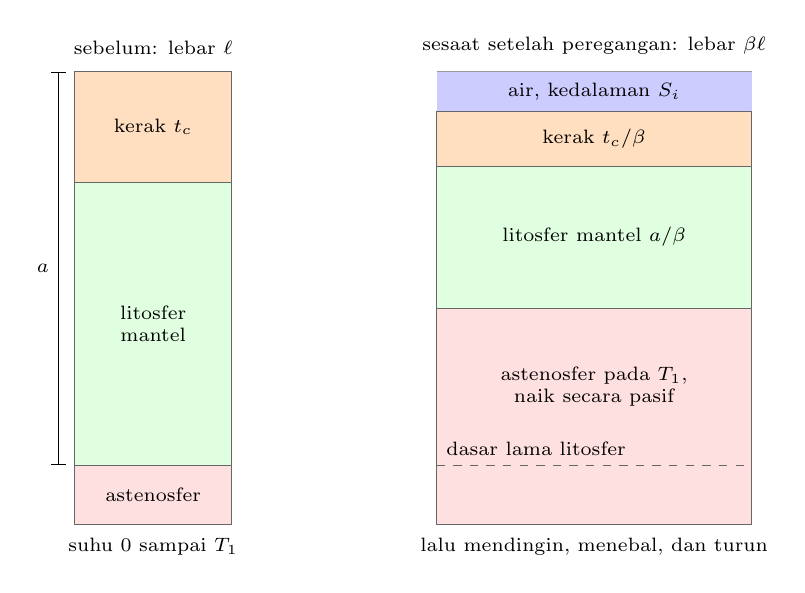
\begin{tikzpicture}[x=0.5cm, y=0.5cm, font=\scriptsize, line join=round]
% before
\begin{scope}
\fill[orange!25, draw=black!60, line width=0.3pt] (0,0) rectangle (4,-2.8);
\fill[green!12, draw=black!60, line width=0.3pt] (0,-2.8) rectangle (4,-10);
\fill[red!12, draw=black!60, line width=0.3pt] (0,-10) rectangle (4,-11.5);
\node at (2,-1.4) {kerak $t_c$};
\node[align=center] at (2,-6.4) {litosfer\\mantel};
\node at (2,-10.75) {astenosfer};
\draw[|-|] (-0.4,0) -- (-0.4,-10) node[midway, left] {$a$};
\node[anchor=south] at (2,0.2) {sebelum: lebar $\ell$};
\node[anchor=north] at (2,-11.6) {suhu $0$ sampai $T_1$};
\end{scope}
% after
\begin{scope}[xshift=4.6cm]
\fill[blue!20] (0,0) rectangle (8,-1.0);
\fill[orange!25, draw=black!60, line width=0.3pt] (0,-1.0) rectangle (8,-2.4);
\fill[green!12, draw=black!60, line width=0.3pt] (0,-2.4) rectangle (8,-6.0);
\fill[red!12, draw=black!60, line width=0.3pt] (0,-6.0) rectangle (8,-11.5);
\draw[black!60, dashed] (0,-10) -- (8,-10);
\node at (4,-0.5) {air, kedalaman $S_i$};
\node at (4,-1.7) {kerak $t_c/\beta$};
\node at (4,-4.2) {litosfer mantel $a/\beta$};
\node[align=center] at (4,-8.0) {astenosfer pada $T_1$,\\naik secara pasif};
\node[anchor=south west] at (0,-10) {dasar lama litosfer};
\node[anchor=south] at (4,0.2) {sesaat setelah peregangan: lebar $\beta\ell$};
\node[anchor=north] at (4,-11.6) {lalu mendingin, menebal, dan turun};
\draw[black!40] (0,0) -- (8,0);
\end{scope}
\end{tikzpicture}
\par\smallskip{\small \omterm{def:b2:basins-compared:stretching}{Model peregangan} (tidak berskala): litosfer setebal $a$ dengan
kerak $t_c$ diregangkan menjadi $\beta$ kali lebarnya; kerak dan litosfer mantel menipis dengan faktor
$\beta$, astenosfer naik, dan permukaan turun sebesar \omterm{def:b2:basins-compared:stretching}{penurunan sin-celah} $S_i$ di bawah
air. Di sini $\beta = 2$.}
\end{omfigure}

\begin{proposition}[Penurunan dalam model peregangan]\label{prop:b2:basins-compared:stretching}
Misalkan litosfer setebal $a$, dengan kerak setebal $t_c$, memiliki geoterm linear dari
$0$ di permukaan sampai suhu astenosfer $T_1$ di dasarnya; misalkan kerak dan mantel
bermassa jenis $\rho_c(1 - \alpha T)$ dan $\rho_m(1 - \alpha T)$, dengan $\alpha$ koefisien
muai termal. Jika litosfer itu diregangkan seketika dengan faktor $\beta$ dan cekungannya terisi
air bermassa jenis $\rho_w$:
\begin{enumerate}
  \item \omterm{def:b2:basins-compared:stretching}{penurunan sin-celahnya} adalah
  \[
    S_i = \frac{a\left(1 - \dfrac{1}{\beta}\right)\left[(\rho_m - \rho_c)\dfrac{t_c}{a}
          \left(1 - \dfrac{\alpha T_1 t_c}{2a}\right) - \dfrac{\alpha T_1 \rho_m}{2}\right]}
          {\rho_m(1 - \alpha T_1) - \rho_w};
  \]
  \item \omterm{def:b2:basins-compared:stretching}{penurunan pascacelah}, selang waktu $t$ setelah peregangan, sampai suku pertama suatu deret, adalah
  \[
    S_t = E_0\,\frac{\beta}{\pi}\sin\frac{\pi}{\beta}\left(1 - e^{-t/\tau}\right),\qquad
    E_0 = \frac{4a\rho_m\alpha T_1}{\pi^2(\rho_m - \rho_w)},\qquad
    \tau = \frac{a^2}{\pi^2\kappa},
  \]
  dengan $\kappa$ difusivitas termal dan $\tau$ \emph{tetapan waktu
  termal}\index{tetapan waktu termal} litosfer.
\end{enumerate}
\end{proposition}
% ledger: pybacktrack:rifting

\begin{proof}
(1) Bandingkan kolom sebelum peregangan dengan kolom sesaat sesudahnya, sampai dasar lama
litosfer, pada kedalaman $a$ di bawah permukaan sebelum peregangan. Sebelumnya, kerak
setebal $t_c$ dan litosfer mantel bersuhu $T = T_1 z/a$; sesudahnya, keduanya
lebih tipis dengan faktor $\beta$ dan suhunya berkisar dari $0$ sampai $T_1$ sepanjang $a/\beta$, sehingga titik
pada kedalaman $z'$ di bawah dasar air bersuhu $T = T_1\beta z'/a$; di bawahnya, astenosfer pada
$T_1$ bermassa jenis $\rho_m(1 - \alpha T_1)$; di atasnya, air mengisi kedalaman $S_i$. Massa
lapisan bermassa jenis $\rho(1 - \alpha T)$ yang suhunya $T$ naik secara linear dari $T_a$ sampai $T_b$ adalah
$\rho\,h\,(1 - \alpha(T_a + T_b)/2)$. Sebelumnya, kolom itu memuat
\[
  \rho_c t_c\left(1 - \frac{\alpha T_1 t_c}{2a}\right)
  + \rho_m (a - t_c)\left(1 - \frac{\alpha T_1 (a + t_c)}{2a}\right);
\]
sesudahnya, kolom itu memuat air, kerak dan litosfer mantel yang menipis, serta astenosfer yang
mengisi sisa kedalaman $a$:
\[
  \rho_w S_i + \frac{\rho_c t_c}{\beta}\left(1 - \frac{\alpha T_1 t_c}{2a}\right)
  + \frac{\rho_m (a - t_c)}{\beta}\left(1 - \frac{\alpha T_1 (a + t_c)}{2a}\right)
  + \rho_m(1 - \alpha T_1)\left(a - S_i - \frac{a}{\beta}\right).
\]
Isostasi membuat keduanya sama. Mengumpulkan suku-suku dalam $S_i$ di satu sisi dan faktor
$(1 - 1/\beta)$ di sisi lain, lalu menjabarkannya, memberikan rumus itu; aljabarnya adalah
\cref{exo:b2:basins-compared:11}.

(2) Setelah peregangan, lempeng mendingin melalui konduksi di antara permukaan yang dijaga pada $0$ dan dasar yang dijaga
pada $T_1$, menuju profil linear tempat ia bermula. Suhu lebihnya memenuhi persamaan
kalor dengan nilai nol di puncak dan dasar, sehingga merupakan jumlah suku-suku
$b_n\sin(n\pi z/a)\,e^{-n^2\kappa\pi^2 t/a^2}$; masing-masing mendingin dengan waktunya sendiri, $\tau/n^2$. Kalor
yang hilang membuat kolom itu menyusut sebesar $\alpha\int \Delta T\,\mathrm{d}z$, dan air tambahan
yang mengisi ruang itu menurunkannya lebih jauh dengan faktor $\rho_m/(\rho_m - \rho_w)$. Hanya suku-suku ganjil yang
berkontribusi; mempertahankan suku pertama, yang koefisiennya dihitung dari profil awal, memberikan
ungkapan itu. Suku-suku lainnya mendingin sembilan kali lebih cepat atau lebih, dan setelah sekitar sepuluh juta tahun
suku-suku itu menggeser penurunan dengan besaran yang hampir tetap, kurang dari \qty{100}{m} untuk $\beta$ dari
1.2 sampai 4 dengan nilai-nilai di bawah.
\end{proof}
% values (script): basins.thermal_series vs basins.thermal, tested in tests/bachelor-2/test_basins.py

Parameter makalah McKenzie adalah $a = \qty{125}{km}$, $T_1 = \qty{1333}{\celsius}$,
$\alpha = \qty{3.28e-5}{K^{-1}}$, $\kappa = \qty{8e-7}{m^2.s^{-1}}$, $\rho_m =
\qty{3330}{kg.m^{-3}}$ (pada \qty{0}{\celsius}), $\rho_c = \qty{2800}{kg.m^{-3}}$; dengan air laut bermassa jenis
\qty{1030}{kg.m^{-3}} parameter itu memberikan $\tau = \qty{62.7}{Ma}$ dan $E_0 = \qty{3207}{m}$. Dengan kerak setebal
\qty{35}{km}, \omterm{def:b2:basins-compared:stretching}{penurunan sin-celahnya} adalah $S_i = \qty{4334}{m} \times (1 - 1/\beta)$.
% ledger: sheplev98:parameters, pybacktrack:rifting
% values (script): tau_Myr 62.7, E0_m 3206.9, Si_max_m 4333.8

\begin{omfigure}
\centering
% figdata/bachelor-2/basins.py part curves
\begin{tikzpicture}
\begin{axis}[width=0.8\linewidth, height=6.2cm, y dir=reverse, xmin=0, xmax=200, ymin=0,
  ymax=6500, xlabel={waktu setelah peregangan (\unit{Ma})},
  ylabel={penurunan tektonik (\unit{m})}, tick label style={font=\scriptsize},
  label style={font=\small}, xtick pos=bottom, ytick pos=left]
\addplot[black!45, line width=1pt] table[x=t_Myr, y=b1.2] {figdata/out/bachelor-2-basins-curves.dat};
\addplot[blue!70!black, line width=1pt] table[x=t_Myr, y=b1.5] {figdata/out/bachelor-2-basins-curves.dat};
\addplot[omThm, line width=1pt] table[x=t_Myr, y=b2] {figdata/out/bachelor-2-basins-curves.dat};
\addplot[orange!80!black, line width=1pt] table[x=t_Myr, y=b4] {figdata/out/bachelor-2-basins-curves.dat};
\node[font=\scriptsize, anchor=south west, inner sep=1pt] at (axis cs:150,1225) {$\beta = 1.2$};
\node[font=\scriptsize, anchor=south west, inner sep=1pt] at (axis cs:150,2595) {$\beta = 1.5$};
\node[font=\scriptsize, anchor=south west, inner sep=1pt] at (axis cs:150,3965) {$\beta = 2$};
\node[font=\scriptsize, anchor=south west, inner sep=1pt] at (axis cs:150,5815) {$\beta = 4$};
\draw[black!40, dashed] (axis cs:62.7,0) -- (axis cs:62.7,6500);
\node[font=\scriptsize, anchor=north west] at (axis cs:63,150) {$t = \tau$};
\end{axis}
\end{tikzpicture}
\par\smallskip{\small Penurunan \omterm{def:b2:basins-compared:stretching}{model peregangan} yang terbebani air untuk empat \omterm{def:b2:basins-compared:stretching}{faktor
peregangan}, dengan kerak \qty{35}{km} dan parameter dalam teks: lompatan sin-celah pada
$t = 0$, lalu kurva pascacelah, yang telah mencapai \qty{63}{\percent} nilai akhirnya pada
$t = \tau$.}
\end{omfigure}

Tiga ciri model itu berlaku pula pada cekungan yang sebenarnya.
\begin{itemize}
  \item Lompatan sin-celah tumbuh bersama $\beta$, demikian pula \omterm{def:b2:basins-compared:stretching}{penurunan pascacelah}; tetapi
        rasionya hampir tidak berubah, sehingga kedua bagian menunjuk ke $\beta$ yang sama jika model itu berlaku.
  \item Skala waktu \omterm{def:b2:basins-compared:stretching}{penurunan pascacelah} tidak bergantung pada $\beta$: skala itu ditentukan oleh
        tebal litosfer saja. Setelah $\tau$, \qty{63}{\percent} penurunan termal
        telah terjadi; setelah $3\tau$, sekitar \qty{95}{\percent}. Celah yang berhenti dua
        ratus juta tahun yang lalu hampir tidak turun lagi.
  \item Suku sin-celah adalah persaingan antara kerak ringan yang menipis, yang membuat
        permukaan turun, dan astenosfer panas yang naik, yang mengapungkannya. Dengan kerak tipis
        yang kedua menang dan peregangan mengangkat permukaan (\cref{exo:b2:basins-compared:10}).
\end{itemize}

Untuk mencocokkan sebuah sumur, penurunan tektonik pada akhir pembentukan celah memberikan $S_i$, sehingga
$\beta = 1/(1 - S_i/\qty{4334}{m})$ untuk kerak \qty{35}{km}; kurva pascacelah lalu diramalkan
dan dibandingkan dengan titik-titik hasil \omterm{def:b2:basins-compared:backstripping}{pengupasan balik} lainnya. Pada sumur rekaan, $S_i = \qty{1441}{m}$
memberikan $\beta = 1.50$, dan kurvanya lewat dalam jarak beberapa meter dari titik-titik kemudian (gambar di
\cref{sec:b2:basins-compared:backstripping}). Cekungan yang sebenarnya jarang semudah itu. Di
Laut Utara bagian tengah, peregangan 50 sampai \qty{100}{\percent} di bagian tengah, $\beta$ dari 1.5 sampai 2,
menghasilkan kembali amplitudo dan laju \omterm{def:b2:basins-compared:stretching}{penurunan pascacelah}. Di tepi Amerika Serikat
bagian timur, hanya satu segmen, Long Island Platform, yang memiliki isian pascacelah awal setebal
yang diramalkan oleh peregangan seragam; di Georges Bank Basin dan Baltimore Canyon Trough
isiannya 1.5 sampai 3 kali lebih tebal, dan penyebab lain pasti ikut bekerja.
% ledger: sc80b4:north-sea, lang24:atlantic

\section{Cekungan dibandingkan}\label{sec:b2:basins-compared:compared}

Tabel di bawah menghimpun keempat keluarga itu. Kurva-kurvanya berbeda dalam bentuk dan skala waktu, dan
\omterm{def:b2:basins-compared:curve}{kurva penurunan} sering menjadi petunjuk pertama tentang sifat cekungan yang terkubur di bawah batuan yang lebih muda.

\begin{center}
\small
\begin{tabular}{>{\raggedright\arraybackslash}p{0.13\linewidth}>{\raggedright\arraybackslash}p{0.19\linewidth}>{\raggedright\arraybackslash}p{0.26\linewidth}>{\raggedright\arraybackslash}p{0.29\linewidth}}
\hline
cekungan & contoh & tebal dan lama & bentuk \omterm{def:b2:basins-compared:curve}{kurva penurunan} tektonik \\
\hline
celah & Laut Utara bagian tengah & graben sejak Trias; peregangan terakhir dari Jura Tengah sampai
pertengahan Kapur; \omterm{def:b2:basins-compared:stretching}{penurunan pascacelah} terbebani air 1.1 sampai \qty{1.4}{km} & lompatan sin-celah yang cepat,
lalu perlambatan eksponensial dengan $\tau$ puluhan juta tahun \\
tepi pasif & Baltimore Canyon Trough & lebih dari \qty{14}{km} sejak Jura & seperti
celah, dengan bagian pascacelah yang besar; isiannya menebal ke arah samudra \\
depan-pegunungan & \omterm{def:b2:alpine-orogen:foreland}{Molasse} Alpen Utara & lebih dari \qty{4}{km} di front sesar dorong, Eosen akhir sampai
Miosen akhir & paling dalam di dekat sabuk dan berpindah bersamanya; bagian dalamnya akhirnya
tertimpa oleh sesar-sesar dorong \\
intrakratonik & Michigan & lebih dari \qty{4}{km} dalam episode-episode selama sekitar 500 Ma & lambat, dengan
episode penurunan yang lebih cepat yang dialami bersama oleh cekungan-cekungan yang berjauhan \\
\hline
\end{tabular}
\end{center}
% ledger: sc80b4:north-sea, schlee76:atlantic, poag79:bct, krenmayr99:molasse, schmid04:foreland, sloss82:michigan

\omterm{def:b2:alpine-orogen:foreland}{Cekungan depan-pegunungan} turun di bawah beban yang bergerak ke arahnya: cekungan itu berpindah bersama sabuk,
cekungan Alpen sejauh sedikitnya \qty{210}{km} di atas kraton Eropa, dan bagian dalamnya
akhirnya tertimpa dan terbawa oleh sesar-sesar dorong, seperti \omterm{def:b2:alpine-orogen:foreland}{Molasse} Subalpin dalam
\cref{ch:b2:alpine-orogen}. \omterm{def:b2:basins-compared:types}{Cekungan celah} melambat selagi mendingin, berapa pun
peregangannya. \omterm{def:b2:basins-compared:types}{Cekungan intrakratonik} turun perlahan dan lama, berdenyut-denyut; baik peregangan
maupun beban tidak menjelaskannya dengan baik, dan karena itulah cekungan ini tetap menjadi pertanyaan penelitian.
% ledger: schmid04:foreland, sinclair97:trinity, krenmayr99:molasse

\begin{inthelab}[Analisis penurunan]
Para analis cekungan mengerjakan isi kotak metode dengan program. Sebuah program sumber terbuka, misalnya,
membaca sebuah lokasi bor sebagai daftar satuan dengan umur, kedalaman, dan litologinya, dan
tabel litologi dengan massa jenis butiran, porositas permukaan, dan panjang peluruhannya. Modul
\omterm{def:b2:basins-compared:backstripping}{pengupasan baliknya} mendekompaksi satuan-satuan itu dan mengembalikan penurunan tektonik pada setiap umur;
karena kedalaman air purba hanya diketahui sebagai rentang, pengguna memberikan nilai minimum dan maksimum dan
program itu mengembalikan kedua penurunan beserta rata-ratanya. Modul kedua bekerja ke arah sebaliknya:
dari model penurunan tektonik, modul itu meramalkan kedalaman air masa lalu, yang dapat
diperiksa terhadap fosil. Para analis lalu mencocokkan \omterm{def:b2:basins-compared:stretching}{faktor peregangan}, menguji kurva muka laut, dan
memetakan penurunan seluruh cekungan dari ratusan atau ribuan sumur.
\end{inthelab}
% ledger: pybacktrack:modules, crowe09:michigan

\section*{Latihan}\label{sec:b2:basins-compared:exercises}

Data untuk latihan, kecuali dinyatakan lain: $\rho_m = \qty{3330}{kg.m^{-3}}$, $\rho_c =
\qty{2800}{kg.m^{-3}}$, $\rho_w = \qty{1030}{kg.m^{-3}}$; \omterm{def:b2:basins-compared:stretching}{model peregangan} dengan $a =
\qty{125}{km}$, $T_1 = \qty{1333}{\celsius}$, $\alpha = \qty{3.28e-5}{K^{-1}}$, $\kappa =
\qty{8e-7}{m^2.s^{-1}}$, $\tau = \qty{62.7}{Ma}$, $E_0 = \qty{3207}{m}$; kerak \qty{35}{km}
memberikan $S_i = \qty{4334}{m}\times(1 - 1/\beta)$; tetapan litologi dalam tabel di
\cref{sec:b2:basins-compared:curves}.

\begin{exercise}[$\star$]\label{exo:b2:basins-compared:1}
Sebutkan keluarga setiap cekungan dan penyebab utama penurunannya: (a) cekungan Michigan;
(b) Laut Utara bagian tengah; (c) Baltimore Canyon Trough; (d) \omterm{def:b2:alpine-orogen:foreland}{Molasse} Alpen Utara;
(e) dataran Indo-Gangga di depan Himalaya.
\end{exercise}

\begin{exercise}[$\star$]\label{exo:b2:basins-compared:2}
Sebuah cekungan menyimpan \qty{3.0}{km} sedimen dengan massa jenis rata-rata \qty{2300}{kg.m^{-3}}. (a) Tentukan
penurunan tektoniknya jika sedimen mencapai muka laut. (b) Dan jika \qty{200}{m} air terletak di
atasnya? (c) Berapa fraksi tebal isian yang disebabkan oleh beban isian itu sendiri?
\end{exercise}

\begin{exercise}[$\star$]\label{exo:b2:basins-compared:3}
Refraksi seismik menunjukkan bahwa kerak \qty{35}{km} telah ditipiskan menjadi \qty{25}{km} di sebuah celah.
(a) Berapa $\beta$? (b) Berapa tebal litosfer sesaat setelah peregangan? (c) Berapa
\omterm{def:b2:basins-compared:stretching}{penurunan sin-celah} di bawah air?
\end{exercise}

\begin{exercise}[$\star$]\label{exo:b2:basins-compared:4}
(a) Periksalah bahwa $\tau = \qty{62.7}{Ma}$ ($1~\text{Ma} = \qty{3.156e13}{s}$). (b) Sebagian program
memakai $\kappa = \qty{1e-6}{m^2.s^{-1}}$: berapa $\tau$ dalam hal itu? (c) Berapa nilainya untuk
litosfer setebal \qty{100}{km}, dengan $\kappa = \qty{8e-7}{m^2.s^{-1}}$? (d) Berapa fraksi
\omterm{def:b2:basins-compared:stretching}{penurunan pascacelah} yang telah terjadi setelah $\tau$, dan setelah $3\tau$?
\end{exercise}

\begin{exercise}[$\star\star$]\label{exo:b2:basins-compared:5}
Sebuah satuan serpih kini terletak di antara \qty{1000}{m} dan \qty{2000}{m}. (a) Tentukan porositasnya di
puncak dan di dasar. (b) Tentukan ketebalan padatnya. (c) Tentukan massanya per satuan luas dan massa jenis
rata-ratanya, dengan pori-pori yang penuh air.
\end{exercise}

\begin{exercise}[$\star\star$]\label{exo:b2:basins-compared:6}
Serpih dari \cref{exo:b2:basins-compared:5} dibawa kembali ke permukaan. (a) Iterasikan
rumus dekompaksi dari $z_2' = T_s$ sampai perubahannya kurang dari \qty{1}{m}. (b) Berapa
massa jenis rata-ratanya di permukaan? (c) Berapa lebih tebal serpih itu?
\end{exercise}

\begin{exercise}[$\star\star$]\label{exo:b2:basins-compared:7}
Di Laut Utara bagian tengah, batuan dasar yang terbebani air turun 1100 sampai \qty{1400}{m} setelah
peregangan yang berakhir pada pertengahan Kapur, sekitar \qty{100}{Ma} yang lalu. (a) Berapa \omterm{def:b2:basins-compared:stretching}{penurunan pascacelah}
yang diberikan model itu setelah \qty{100}{Ma} untuk $\beta = 1.5$ dan $\beta = 2$? (b) Apakah
nilai-nilai itu mengapit pengamatan? (c) Untuk $\beta$ berapa model itu memberikan \qty{1250}{m}?
Gunakan $\frac{\beta}{\pi}\sin\frac{\pi}{\beta} = 0.4705$ untuk $\beta = 1.6$ dan $0.5204$ untuk $\beta
= 1.7$ lalu interpolasikan.
\end{exercise}

\begin{exercise}[$\star\star$]\label{exo:b2:basins-compared:8}
Cekungan sin-celah suatu \omterm{def:b2:basins-compared:stretching}{model peregangan} tidak terisi air tetapi sedimen bermassa jenis
\qty{2300}{kg.m^{-3}}. (a) Dalam rumus $S_i$, apa yang berubah? (b) Hitunglah $S_i$ yang terbebani sedimen
untuk $\beta = 1.5$ dengan kerak \qty{35}{km}, jika diketahui pembilang rumus itu
$a(1 - 1/\beta)\times\qty{74.69}{kg.m^{-3}}$ dan $\rho_m(1 - \alpha T_1) =
\qty{3184.4}{kg.m^{-3}}$. (c) Bandingkan dengan nilai yang terbebani air.
\end{exercise}

\begin{exercise}[$\star\star$]\label{exo:b2:basins-compared:9}
Sebuah sumur yang dikupas balik memberikan $Y = \qty{2171}{m}$ pada \qty{100}{Ma}, dengan anggapan muka laut kini. (a)
Jika muka laut saat itu \qty{100}{m} lebih tinggi, berapa $Y$? (b) Jika fosil memberikan kedalaman air
di antara 100 dan \qty{500}{m} alih-alih \qty{300}{m}, rentang $Y$ berapa yang diperoleh? (c) Manakah dari
kedua ketidakpastian itu yang lebih besar?
\end{exercise}

\begin{exercise}[$\star\star\star$]\label{exo:b2:basins-compared:10}
(a) Tunjukkan dari \cref{prop:b2:basins-compared:stretching} bahwa peregangan membuat permukaan naik
alih-alih turun bila $(\rho_m - \rho_c)\frac{t_c}{a}\left(1 - \frac{\alpha T_1 t_c}{2a}\right) <
\frac{\alpha T_1\rho_m}{2}$. (b) Dengan mengabaikan suku kecil $\alpha T_1 t_c/(2a)$, tentukan
tebal kerak kritis. (c) Perhalus nilai itu dengan satu iterasi. (d) Di mana di Bumi kamu akan mencari
celah yang naik selagi membuka?
\end{exercise}

\begin{exercise}[$\star\star\star$]\label{exo:b2:basins-compared:11}
(a) Tuliskan keseimbangan isostatik dalam bukti \cref{prop:b2:basins-compared:stretching}, bagian
(1), dan turunkan rumus $S_i$. (b) Tunjukkan bahwa \omterm{def:b2:basins-compared:stretching}{penurunan pascacelah} akhir yang eksak, ketika
lempeng telah kembali ke geoterm linearnya, adalah $\alpha\rho_m T_1 a(1 - 1/\beta)/(2(\rho_m -
\rho_w))$. (c) Hitunglah nilainya untuk $\beta = 2$ dan bandingkan dengan nilai akhir
rumus suku pertama.
\end{exercise}

\begin{exercise}[$\star\star\star$]\label{exo:b2:basins-compared:12}
Sebuah tepi pasif diregangkan dengan $\beta = 2$ dan telah mendingin selama \qty{150}{Ma}; cekungannya
tetap penuh sedimen dengan massa jenis rata-rata \qty{2400}{kg.m^{-3}} sampai muka laut.
(a) Tentukan \omterm{def:b2:basins-compared:stretching}{penurunan pascacelah} yang terbebani air. (b) Berapa tebal sedimen pascacelah?
(c) Di Baltimore Canyon Trough isian pascacelah awal 1.5 sampai 3 kali lebih tebal daripada
yang diramalkan peregangan seragam: tebal berapa artinya di sini? (d) Ajukan penyebab-penyebabnya.
\end{exercise}

\begin{problem}[{Soal akhir pekan --- Pengupasan balik sebuah sumur}]\label{pb:b2:basins-compared:1}
Di Cekungan Kestrel yang rekaan, sebuah sumur mengambil inti empat satuan. Dari dasar: pasir yang diendapkan selama
pembentukan celah, dari 165 sampai \qty{150}{Ma}, kini di antara \qty{4420}{m} dan \qty{6030}{m}; serpih, 150
sampai \qty{100}{Ma}, di antara \qty{3310}{m} dan \qty{4420}{m}; kapur, 100 sampai \qty{60}{Ma}, di antara
\qty{1700}{m} dan \qty{3310}{m}; pasir lempungan, \qty{60}{Ma} sampai kini, di antara \qty{0}{m} dan
\qty{1700}{m} di bawah dasar laut. Fosil memberikan kedalaman air di puncak setiap satuan ketika satuan itu
diendapkan: \qty{200}{m} pada \qty{150}{Ma}, \qty{300}{m} pada \qty{100}{Ma}, \qty{150}{m} pada
\qty{60}{Ma}; kini kedalamannya \qty{100}{m}. Gunakan tabel litologi bab ini, $\rho_m =
\qty{3330}{kg.m^{-3}}$ dan $\rho_w = \qty{1030}{kg.m^{-3}}$ untuk air laut maupun air pori, muka laut
seperti kini, dan \omterm{def:b2:basins-compared:stretching}{model peregangan} bab ini dengan kerak \qty{35}{km}. Kedalaman dibulatkan sampai
meter.

\noindent\textbf{Bagian I --- Pemadatan.}
\begin{enumerate}
  \item Tentukan porositas pasir di puncak dan di dasarnya kini.
  \item Tentukan ketebalan padat pasir itu.
  \item Ketebalan padat serpih, kapur, dan pasir lempungan adalah \qty{1011}{m},
        \qty{1409}{m} dan \qty{1004}{m}. Periksalah salah satunya.
  \item Tentukan massa per satuan luas setiap satuan kini, lalu massa jenis rata-rata seluruh
        kolom.
  \item Pada \qty{150}{Ma} pasir itu terletak di dasar laut. Dekompaksilah: iterasikan dari $z_2' =
        T_s$ sampai perubahannya kurang dari \qty{1}{m}.
  \item Tentukan massa jenis rata-rata pasir yang telah didekompaksi.
\end{enumerate}

\noindent\textbf{Bagian II --- Pengupasan balik.}
\begin{enumerate}[resume]
  \item Tentukan penurunan tektonik $Y$ pada \qty{150}{Ma}.
  \item Tentukan penurunan tektonik kini. Mengapa tidak diperlukan dekompaksi?
  \item Sebuah program memberikan $Y = \qty{2171}{m}$ pada \qty{100}{Ma} dan $Y = \qty{2453}{m}$ pada
        \qty{60}{Ma}. Hitunglah laju rata-rata penurunan tektonik dalam masing-masing dari ketiga
        selang sejak \qty{150}{Ma}.
  \item Tentukan penurunan total kini dan bandingkan dengan penurunan tektonik.
  \item Berapa fraksi kedalaman batuan dasar kini yang disebabkan oleh beban sedimen?
  \item Jika muka laut pada \qty{100}{Ma} berada \qty{100}{m} lebih tinggi daripada kini, berapa $Y$
        saat itu?
\end{enumerate}

\noindent\textbf{Bagian III --- Mencocokkan model peregangan.} Pembentukan celah dianggap seketika
dan berakhir pada \qty{150}{Ma}.
\begin{enumerate}[resume]
  \item Titik mana pada kurva yang memberikan \omterm{def:b2:basins-compared:stretching}{penurunan sin-celah}?
  \item Tentukan \omterm{def:b2:basins-compared:stretching}{faktor peregangan} $\beta$, sampai dua desimal.
  \item Berapa tebal kerak dan litosfer sesaat setelah peregangan?
  \item Dengan $\beta$ yang dibulatkan, hitunglah $\frac{\beta}{\pi}\sin\frac{\pi}{\beta}$ dan \omterm{def:b2:basins-compared:stretching}{penurunan
        pascacelah} akhir.
  \item Ramalkan $Y$ pada 100, 60, dan \qty{0}{Ma}.
  \item Bandingkan dengan nilai-nilai hasil \omterm{def:b2:basins-compared:backstripping}{pengupasan balik}.
  \item Kecocokannya dekat karena sumur itu rekaan. Berikan tiga alasan mengapa sumur yang sebenarnya
        tidak akan cocok sebaik itu.
\end{enumerate}

\noindent\textbf{Bagian IV --- 50 juta tahun berikutnya.}
\begin{enumerate}[resume]
  \item Berapa banyak lagi penurunan tektonik yang akan terjadi dalam \qty{50}{Ma} berikutnya?
  \item Jika kedalaman air tetap \qty{100}{m}, berapa banyak sedimen bermassa jenis
        \qty{2400}{kg.m^{-3}} yang dapat terakumulasi dalam waktu itu?
  \item Berapa fraksi \omterm{def:b2:basins-compared:stretching}{penurunan pascacelah} akhir yang telah dialami cekungan itu?
  \item Kapan separuhnya telah terjadi?
  \item Sebagai ringkasan: \omterm{def:b2:basins-compared:stretching}{faktor peregangan} berapa yang direkam sumur itu?
\end{enumerate}
\end{problem}
